\chapter{Excitonic Effects}
\section{Introduction}
The bandstructure and optical properties of semiconductors discussed so far have been based on the assumption that the valence band is completely filled with electrons while the conduction band remains empty. Under this assumption, the effects of carriers—electrons in the conduction band and holes in the valence band—enter only through the occupation probabilities, without altering the underlying bandstructure.\\
In practice, however, there exists a Coulombic interaction between electrons and other charged carriers, such as additional electrons or holes. These interactions can lead to significant modifications in material properties. Let us now consider a situation in which a single electron occupies the conduction band, while a corresponding hole is present in the valence band. This configuration introduces a direct Coulomb attraction between the electron and hole, altering the Hamiltonian of the system.\\
The resultant electron–hole pair, bound by this Coulomb interaction, forms a new quasiparticle known as an exciton. The formation of an exciton necessitates a re-evaluation of the electronic bandstructure to incorporate the effects of this binding.\\
The study of excitonic transitions in quantum wells has emerged as a major area of research, driven by both fundamental physics and technological applications. In quantum confined systems, the exciton binding energy is significantly enhanced compared to bulk materials. Additionally, the strength of optical transitions is improved, leading to the observation of sharp resonance features in the optical spectra of quantum wells. These excitonic resonances are highly tunable using optical or electronic methods, making them especially valuable in device applications.\\
Modulation of optical properties is a critical component in the development of advanced optoelectronic technologies. Although several types of external stimuli—such as electric fields, magnetic fields, and mechanical strain—can influence the optical response of a material, only modulation by electric or electromagnetic fields can achieve high-speed performance. In bulk semiconductors, the modulation capabilities are generally limited. However, quantum wells exhibit markedly enhanced modulation behavior, which makes them ideal candidates for integrated photonic and optoelectronic systems.\\
In this chapter, we will explore the physical principles underlying various approaches to optical modulation, with a particular focus on quantum-confined systems.


\section{Excitonic States in Semiconductors}
The electron–hole pair forms a bound state that can be described by an envelope function. This envelope function, representing the spatial distribution of the bound state, can be derived by treating the Coulombic interaction between the electron and hole as a perturbation.\\
There are two major categories of excitons, distinguished by the spatial extent of their envelope functions. When the envelope function is confined to only a few unit cells, the exciton is referred to as a Frenkel exciton. Owing to their highly localized nature, the Heisenberg uncertainty principle implies that such excitons require a treatment that incorporates the full electronic bandstructure of the material.\\
These localized excitons contrast with another class—commonly encountered in semiconductors—where the envelope function is much more extended. Each class of exciton gives rise to different optical and transport properties and must be described using appropriate theoretical frameworks.
\begin{center}
	\begin{minipage}{0.8\textwidth}
		\centering
		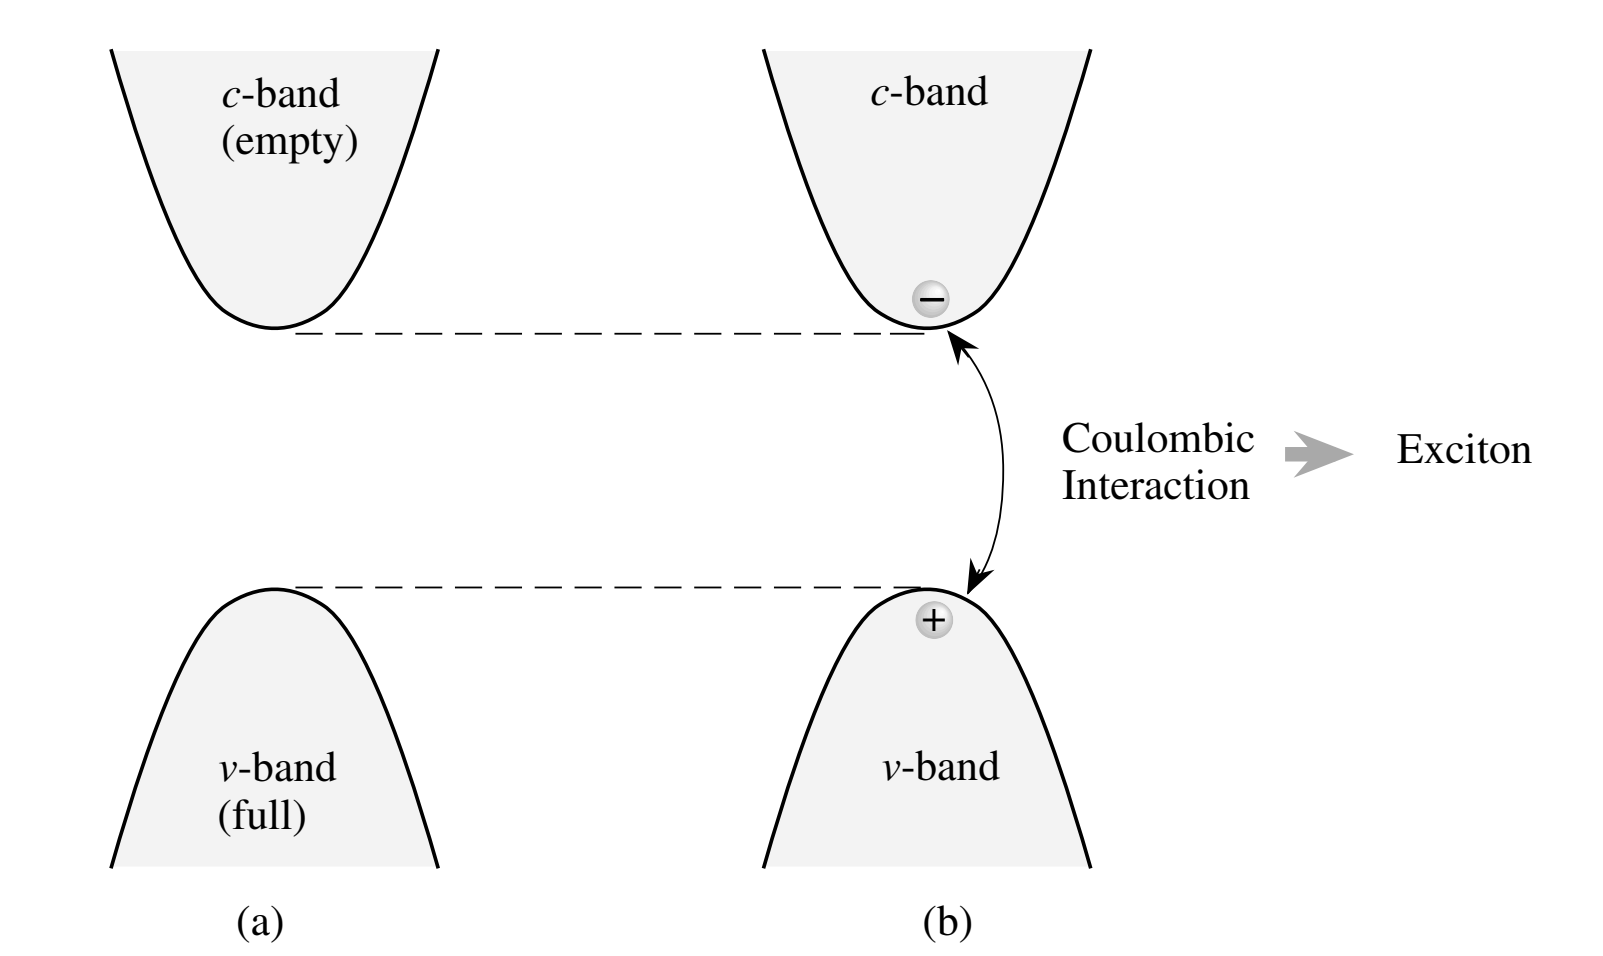
\includegraphics[width=\textwidth]{img/hole_interaction.png}
		\\[0.5em]
		\refstepcounter{figure}
		\textbf{Figure~\thefigure.} (a) Bandstructure under the independent electron approximation.
		(b) Modification of the bandstructure due to Coulomb interaction between an electron and a hole.
		\label{fig:hole_interaction}
	\end{minipage}
\end{center}
\begin{center}
	\begin{minipage}{0.75\textwidth}
		\centering
		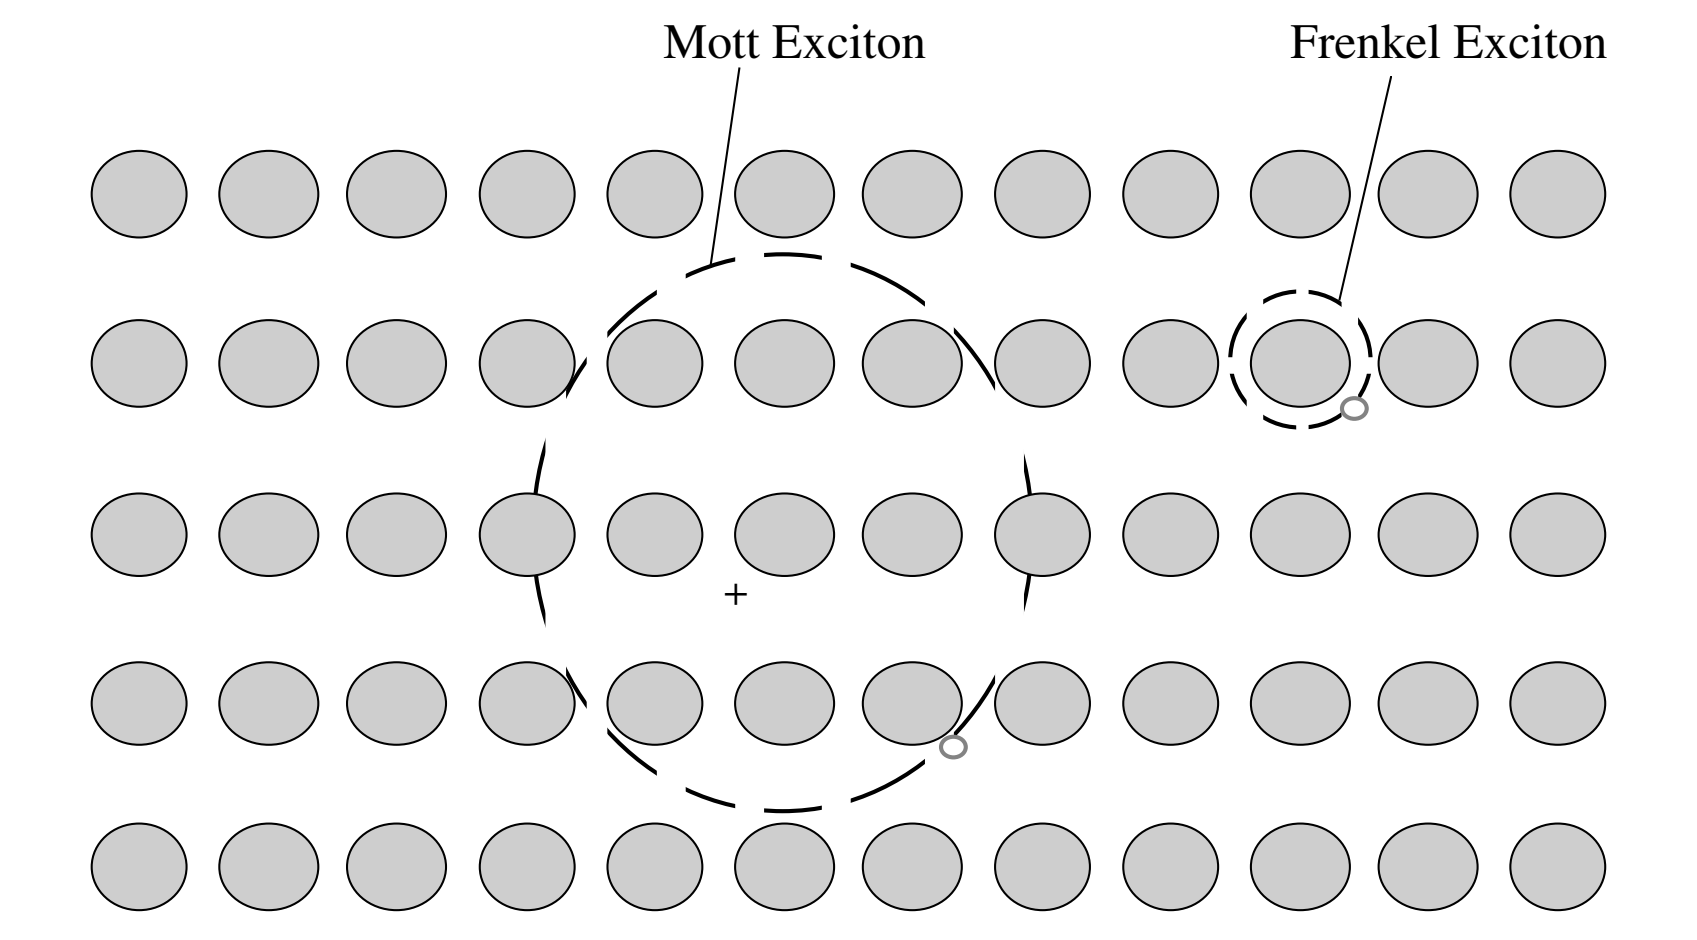
\includegraphics[width=\textwidth]{img/exciton.png}
		\\[0.5em]
		\refstepcounter{figure}
		\textbf{Figure~\thefigure.} Conceptual illustration of the periodic envelope functions of Frenkel and Mott excitons. The Frenkel exciton is localized over a few unit cells, while the Mott exciton extends across many unit cells.
		\label{fig:exciton}
	\end{minipage}
\end{center}

Such excitons, which arise when the electron and hole form a spatially extended bound state, are referred to as Mott excitons. These excitons are central to the excitonic physics in semiconductors. Their properties can be described using the effective mass approximation, whereby the electron–hole interaction is incorporated into a modified Schrödinger equation of the form:
\begin{equation}
	\left[- \frac{\hbar^2}{2m_e^*} \nabla_e^2 - \frac{\hbar^2}{2m_h^*} \nabla_h^2 - \frac{e^2}{4\pi \varepsilon | \mathbf{r}_e - \mathbf{r}_h |} \psi_{ex} \right] = E \psi_{ex}
\end{equation}
Here, \( m_e^* \) and \( m_h^* \) are the effective masses of the electron and hole, respectively, and \( |\mathbf{r}_e - \mathbf{r}_h| \) denotes the distance between the electron and hole, which determines the strength of their Coulomb interaction. \( E_{\text{ex}} \) is the energy of the exciton.
This formulation presents a two-body problem, which can be simplified by transforming to center-of-mass and relative coordinates:
\begin{equation}
	\mathbf{r} = \mathbf{r}_e - \mathbf{r}_h, \quad \mathbf{R} = \frac{m_e^* \mathbf{r}_e + m_h^* \mathbf{r}_h}{m_e^* + m_h^*}
\end{equation}
and corresponding wavevectors:
\begin{equation}
	\mathbf{k} = \frac{m_e^* \mathbf{k}_e + m_h^* \mathbf{k}_h}{m_e^* + m_h^*}, \quad \mathbf{K} = \mathbf{k}_e + \mathbf{k}_h
\end{equation}
The total Hamiltonian can then be written as:
\begin{equation}
	H = \frac{\hbar^2 K^2}{2(m_e^* + m_h^*)} +  \left( \frac{\hbar^2 k^2}{2 m_r^*} - \frac{e^2}{4\pi \varepsilon |\mathbf{r}|} \right)
\end{equation}
The Hamiltonian consists of two parts: the first term describes the center-of-mass motion, which leads to a plane-wave solution:
\begin{equation}
	\psi_{\text{cm}}(\mathbf{R}) = e^{i \mathbf{K} \cdot \mathbf{R}}
\end{equation}
The second term describes the relative motion of the electron–hole pair. Its solution satisfies:
\begin{equation}
	\left[ - \frac{\hbar^2 k^2}{2m_r^*} - \frac{e^2}{4\pi \varepsilon |\mathbf{r}|} \right] F(\mathbf{r}) = E_n F(\mathbf{r})
\end{equation}
This equation is analogous to the hydrogen atom problem, and its solutions \( F(\mathbf{r}) \) are hydrogen-like wavefunctions. The full exciton wavefunction is then:
\begin{equation}
	\psi_{n,\mathbf{K}_{ex}}(\mathbf{r}_e, \mathbf{r}_h) = e^{i \mathbf{K}_{ex} \cdot \mathbf{R}} F_n(\mathbf{r}) \phi_c(\mathbf{r}_e) \phi_v(\mathbf{r}_h)
\end{equation}
Here, \( \phi_c \) and \( \phi_v \) represent the Bloch functions of the conduction and valence band edge states, respectively. The corresponding excitonic energy levels are given by:
\begin{equation}
	E_{n,\mathbf{K}_{ex}} = E_n + \frac{\hbar^2}{2(m_e^* + m_h^*)} K_{ex}^2
\end{equation}
where the eigenvalues \( E_n \) are:
\begin{equation}
	E_n = - \frac{m_r^* e^4}{2 (4 \pi \varepsilon)^2 \hbar^2 n^2}, \quad n = 1, 2, 3, \dots
\end{equation}
The quantity \( E_n \) is measured relative to the conduction band minimum, i.e., the excitonic energy levels appear just below the bandgap. Typical binding energies for excitons in semiconductors range from approximately 2 to 6~meV.\\
This modified dispersion relation, which includes the Coulomb interaction, differs from the conventional energy–wavevector (\( E \) vs.\ \( k \)) relationship. Since the exciton is a composite particle, the appropriate quantum number is not the electron or hole momentum individually, but the total crystal momentum \( \mathbf{K} \) of the electron–hole pair. When the Coulomb interaction is neglected, the bound-state energy levels vanish, and one recovers the usual free electron–hole dispersion relation.\\
A key consequence of excitonic formation is that, unlike in free-carrier models where the joint density of states begins at the band edge, the presence of excitons introduces a density of states below the bandgap. Nevertheless, due to momentum conservation, not all exciton states will couple effectively to photons.
\begin{center}
	\begin{minipage}{0.6\textwidth}
		\centering
		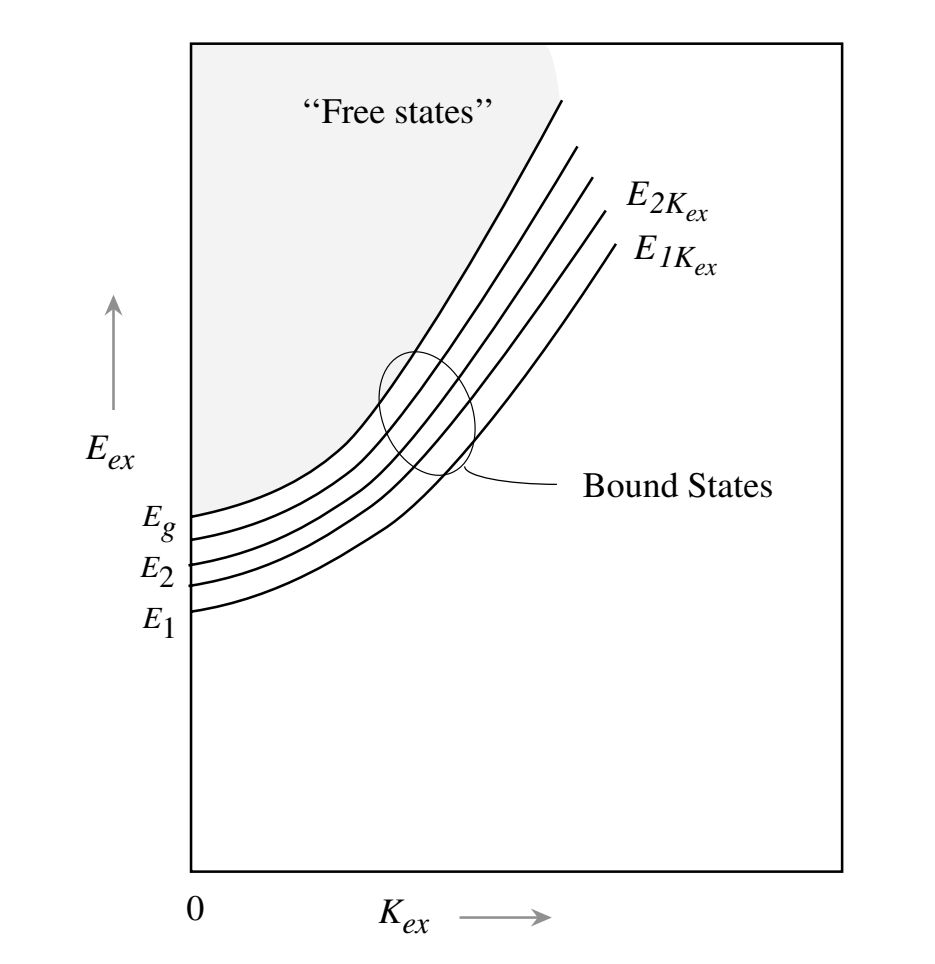
\includegraphics[width=\textwidth]{img/Dispersion_curves.png}
		\\[0.5em]
		\refstepcounter{figure}
		\textbf{Figure~\thefigure.} Dispersion curves for the electron-hole system in the exciton framework
		\label{fig:Dispersion_curves}
	\end{minipage}
\end{center}
To analyze the absorption spectra of excitonic transitions in semiconductors, it is useful to examine the problem in greater detail. As previously discussed, the independent-electron model yields the conduction and valence band states. When electron–hole pairs are introduced, their mutual Coulomb interaction can be treated as a perturbation. The resulting excitonic wavefunction can then be expressed as a linear combination of the independent electron basis functions.\\
The general form of the excitonic Hamiltonian is given by:
\begin{equation}
	H = H_0 + \frac{1}{2} \sum_{i \neq j} \frac{e^2}{4\pi \varepsilon_0 |\mathbf{r}_i - \mathbf{r}_j|}
\end{equation}
Here, \( H_0 \) is the unperturbed Hamiltonian representing the independent electron bandstructure, and the second term accounts for the Coulomb interactions between different electrons. The factor of \( \frac{1}{2} \) prevents double counting. Indices \( i \) and \( j \) label individual particles.\\
Because the full Hamiltonian maintains the symmetry of the underlying crystal lattice, the Bloch theorem remains applicable. Therefore, the total excitonic wavefunction must satisfy:
\begin{equation}
	\psi_{\text{ex}}(\mathbf{r}_1 + \mathbf{R}, \mathbf{r}_2 + \mathbf{R}, \dots) = e^{i\mathbf{K} \cdot \mathbf{R}} \psi_{\text{ex}}(\mathbf{r}_1, \mathbf{r}_2, \dots)
\end{equation}
where \( \mathbf{R} \) is a lattice vector and \( \mathbf{K} \) is the total crystal momentum of the exciton.
The exciton state can be written in terms of a basis function \( \Phi_{c,\mathbf{k_e}, S_e; v,\mathbf{k_h}, S_h} \), which represents a conduction band state where an electron, with momentum \(\mathbf{k}_e\) and spin \(S_e\) in the conduction band, and a valence band hole with momentum \(\mathbf{k}_h\) and spin \(S_h\). The difference \( \mathbf{k}_e - \mathbf{k}_h \) is equal to the total momentum \( \mathbf{K} \) of the exciton.\\
The exciton wavefunction is expressed as:
\begin{equation}
	\psi_{\text{ex}}^{n,\ell,m} = \sum_{\mathbf{k}} A_{n,\ell,m}(\mathbf{k}) \Phi^{n,\ell,m}_{c,\mathbf{k}+\mathbf{K}_{ex}/2,S_e; v,\mathbf{k}-\mathbf{K}_{ex}/2,S_h}
\end{equation}
Here, \( n \), \( \ell \), and \( m \) are quantum numbers associated with the exciton state, and \( A_{n,\ell,m}(\mathbf{k}) \) are expansion coefficients. Since we are dealing with envelope functions that are spatially extended (on the order of 100~\AA), the expansion coefficients are expected to be sharply localized in momentum space.\\
We can define the Fourier transform of \( A_{n,\ell,m}(\mathbf{k}) \) as the real-space envelope function:
\begin{equation}
	F_{n,\ell,m}(\mathbf{r}) = \sum_{\mathbf{k}} A_{n,\ell,m}(\mathbf{k}) e^{i \mathbf{k} \cdot \mathbf{r}}
\end{equation}
This function satisfies a Schrödinger-like equation, analogous to the hydrogen atom, but modified for the semiconductor environment:
\begin{equation}
	\left[ E_{cv}(-i\nabla, \mathbf{K}_{ex}) - \frac{e^2}{4\pi \varepsilon \mathbf{r}} \right] F_{n,\ell,m}(\mathbf{r}) = E_{\text{ex}} F_{n,\ell,m}(\mathbf{r})
\end{equation}
Here, \( E_{cv}(-i\nabla, \mathbf{K}_{ex}) \) results from expanding the difference \( E_c(\mathbf{k} + \mathbf{K}_{ex}/2) - E_v(\mathbf{k} - \mathbf{K}_{ex}/2) \) in powers of \( \mathbf{k} \) and substituting \( \mathbf{k} \rightarrow -i\nabla \). Exchange interactions are typically negligible and are therefore omitted. At low carrier densities, the dielectric constant \( \varepsilon \) can be approximated by its static value.\\
For a simple parabolic band structure, the exciton binding energy levels are:
\begin{equation}
	E^{\text{ex}}_n = E_g - \frac{m_r^*e^4}{2(4\pi \varepsilon)^2 \hbar^2 n^2} = E_g - \frac{R_{\text{ex}}}{n^2}
\end{equation}
where \( m_r^* \) is the reduced mass of the electron–hole pair and \( R_{\text{ex}} \) is the exciton Rydberg. The kinetic energy associated with the center-of-mass motion of the exciton should be added to this expression for the total energy.\\
The corresponding envelope functions are hydrogen-like. For example, the ground state wavefunction is:
\begin{equation}
	F_{100}(\mathbf{r}) = \frac{1}{\sqrt{\pi a_{\text{ex}}^3}} e^{-r/a_{\text{ex}}}
\end{equation}
with the exciton Bohr radius given by:
\begin{equation}
	a_{\text{ex}} = \frac{\varepsilon m_0}{\varepsilon_0 m_r^*} a_B, \quad \text{where } a_B = 0.529\,\text{\AA}
\end{equation}
For most semiconductors, \( a_{\text{ex}} \) is on the order of 100~\AA, indicating that the exciton is spread over many unit cells. This justifies the use of the effective mass approximation in the description of such extended excitonic states.
\begin{center}
	\begin{minipage}{0.8\textwidth}
		\centering
		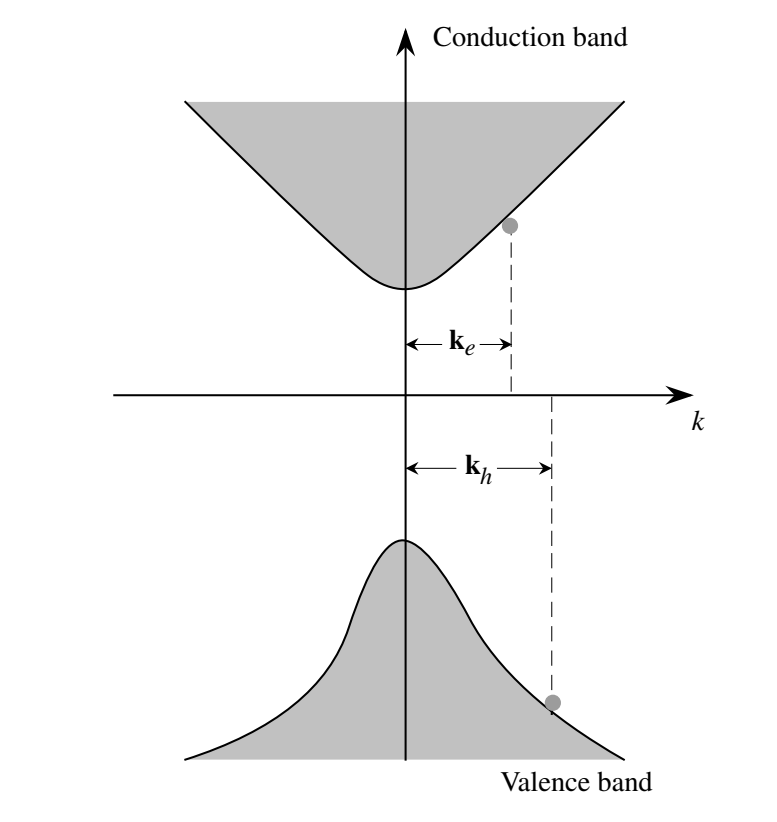
\includegraphics[width=\textwidth]{img/Exciton_Block.png}
		\\[0.5em]
		\refstepcounter{figure}
		\textbf{Figure~\thefigure.} Schematic picture of an exciton in the Bloch representation.
		\label{fig:Exciton_Block}
	\end{minipage}
\end{center}